\documentclass[]{ctexbook}
\usepackage{lmodern}
\usepackage{amssymb,amsmath}
\usepackage{ifxetex,ifluatex}
\usepackage{fixltx2e} % provides \textsubscript
\ifnum 0\ifxetex 1\fi\ifluatex 1\fi=0 % if pdftex
  \usepackage[T1]{fontenc}
  \usepackage[utf8]{inputenc}
\else % if luatex or xelatex
  \ifxetex
    \usepackage{xltxtra,xunicode}
  \else
    \usepackage{fontspec}
  \fi
  \defaultfontfeatures{Ligatures=TeX,Scale=MatchLowercase}
\fi
% use upquote if available, for straight quotes in verbatim environments
\IfFileExists{upquote.sty}{\usepackage{upquote}}{}
% use microtype if available
\IfFileExists{microtype.sty}{%
\usepackage{microtype}
\UseMicrotypeSet[protrusion]{basicmath} % disable protrusion for tt fonts
}{}
\usepackage[b5paper,tmargin=2.5cm,bmargin=2.5cm,lmargin=3.5cm,rmargin=2.5cm]{geometry}
\usepackage[unicode=true]{hyperref}
\PassOptionsToPackage{usenames,dvipsnames}{color} % color is loaded by hyperref
\hypersetup{
            pdftitle={Overleaf功能介绍},
            pdfauthor={wang},
            colorlinks=true,
            linkcolor=Maroon,
            citecolor=Blue,
            urlcolor=Blue,
            breaklinks=true}
\urlstyle{same}  % don't use monospace font for urls
\usepackage{natbib}
\bibliographystyle{apalike}
\usepackage{color}
\usepackage{fancyvrb}
\newcommand{\VerbBar}{|}
\newcommand{\VERB}{\Verb[commandchars=\\\{\}]}
\DefineVerbatimEnvironment{Highlighting}{Verbatim}{commandchars=\\\{\}}
% Add ',fontsize=\small' for more characters per line
\usepackage{framed}
\definecolor{shadecolor}{RGB}{248,248,248}
\newenvironment{Shaded}{\begin{snugshade}}{\end{snugshade}}
\newcommand{\AlertTok}[1]{\textcolor[rgb]{0.94,0.16,0.16}{#1}}
\newcommand{\AnnotationTok}[1]{\textcolor[rgb]{0.56,0.35,0.01}{\textbf{\textit{#1}}}}
\newcommand{\AttributeTok}[1]{\textcolor[rgb]{0.77,0.63,0.00}{#1}}
\newcommand{\BaseNTok}[1]{\textcolor[rgb]{0.00,0.00,0.81}{#1}}
\newcommand{\BuiltInTok}[1]{#1}
\newcommand{\CharTok}[1]{\textcolor[rgb]{0.31,0.60,0.02}{#1}}
\newcommand{\CommentTok}[1]{\textcolor[rgb]{0.56,0.35,0.01}{\textit{#1}}}
\newcommand{\CommentVarTok}[1]{\textcolor[rgb]{0.56,0.35,0.01}{\textbf{\textit{#1}}}}
\newcommand{\ConstantTok}[1]{\textcolor[rgb]{0.00,0.00,0.00}{#1}}
\newcommand{\ControlFlowTok}[1]{\textcolor[rgb]{0.13,0.29,0.53}{\textbf{#1}}}
\newcommand{\DataTypeTok}[1]{\textcolor[rgb]{0.13,0.29,0.53}{#1}}
\newcommand{\DecValTok}[1]{\textcolor[rgb]{0.00,0.00,0.81}{#1}}
\newcommand{\DocumentationTok}[1]{\textcolor[rgb]{0.56,0.35,0.01}{\textbf{\textit{#1}}}}
\newcommand{\ErrorTok}[1]{\textcolor[rgb]{0.64,0.00,0.00}{\textbf{#1}}}
\newcommand{\ExtensionTok}[1]{#1}
\newcommand{\FloatTok}[1]{\textcolor[rgb]{0.00,0.00,0.81}{#1}}
\newcommand{\FunctionTok}[1]{\textcolor[rgb]{0.00,0.00,0.00}{#1}}
\newcommand{\ImportTok}[1]{#1}
\newcommand{\InformationTok}[1]{\textcolor[rgb]{0.56,0.35,0.01}{\textbf{\textit{#1}}}}
\newcommand{\KeywordTok}[1]{\textcolor[rgb]{0.13,0.29,0.53}{\textbf{#1}}}
\newcommand{\NormalTok}[1]{#1}
\newcommand{\OperatorTok}[1]{\textcolor[rgb]{0.81,0.36,0.00}{\textbf{#1}}}
\newcommand{\OtherTok}[1]{\textcolor[rgb]{0.56,0.35,0.01}{#1}}
\newcommand{\PreprocessorTok}[1]{\textcolor[rgb]{0.56,0.35,0.01}{\textit{#1}}}
\newcommand{\RegionMarkerTok}[1]{#1}
\newcommand{\SpecialCharTok}[1]{\textcolor[rgb]{0.00,0.00,0.00}{#1}}
\newcommand{\SpecialStringTok}[1]{\textcolor[rgb]{0.31,0.60,0.02}{#1}}
\newcommand{\StringTok}[1]{\textcolor[rgb]{0.31,0.60,0.02}{#1}}
\newcommand{\VariableTok}[1]{\textcolor[rgb]{0.00,0.00,0.00}{#1}}
\newcommand{\VerbatimStringTok}[1]{\textcolor[rgb]{0.31,0.60,0.02}{#1}}
\newcommand{\WarningTok}[1]{\textcolor[rgb]{0.56,0.35,0.01}{\textbf{\textit{#1}}}}
\usepackage{longtable,booktabs}
% Fix footnotes in tables (requires footnote package)
\IfFileExists{footnote.sty}{\usepackage{footnote}\makesavenoteenv{long table}}{}
\usepackage{graphicx,grffile}
\makeatletter
\def\maxwidth{\ifdim\Gin@nat@width>\linewidth\linewidth\else\Gin@nat@width\fi}
\def\maxheight{\ifdim\Gin@nat@height>\textheight\textheight\else\Gin@nat@height\fi}
\makeatother
% Scale images if necessary, so that they will not overflow the page
% margins by default, and it is still possible to overwrite the defaults
% using explicit options in \includegraphics[width, height, ...]{}
\setkeys{Gin}{width=\maxwidth,height=\maxheight,keepaspectratio}
\IfFileExists{parskip.sty}{%
\usepackage{parskip}
}{% else
\setlength{\parindent}{0pt}
\setlength{\parskip}{6pt plus 2pt minus 1pt}
}
\setlength{\emergencystretch}{3em}  % prevent overfull lines
\providecommand{\tightlist}{%
  \setlength{\itemsep}{0pt}\setlength{\parskip}{0pt}}
\setcounter{secnumdepth}{5}
% Redefines (sub)paragraphs to behave more like sections
\ifx\paragraph\undefined\else
\let\oldparagraph\paragraph
\renewcommand{\paragraph}[1]{\oldparagraph{#1}\mbox{}}
\fi
\ifx\subparagraph\undefined\else
\let\oldsubparagraph\subparagraph
\renewcommand{\subparagraph}[1]{\oldsubparagraph{#1}\mbox{}}
\fi

% set default figure placement to htbp
\makeatletter
\def\fps@figure{htbp}
\makeatother

\usepackage{booktabs}
\usepackage{longtable}

\usepackage{framed,color}
\definecolor{shadecolor}{RGB}{248,248,248}

\renewcommand{\textfraction}{0.05}
\renewcommand{\topfraction}{0.8}
\renewcommand{\bottomfraction}{0.8}
\renewcommand{\floatpagefraction}{0.75}

\let\oldhref\href
\renewcommand{\href}[2]{#2\footnote{\url{#1}}}

\makeatletter
\newenvironment{kframe}{%
\medskip{}
\setlength{\fboxsep}{.8em}
 \def\at@end@of@kframe{}%
 \ifinner\ifhmode%
  \def\at@end@of@kframe{\end{minipage}}%
  \begin{minipage}{\columnwidth}%
 \fi\fi%
 \def\FrameCommand##1{\hskip\@totalleftmargin \hskip-\fboxsep
 \colorbox{shadecolor}{##1}\hskip-\fboxsep
     % There is no \\@totalrightmargin, so:
     \hskip-\linewidth \hskip-\@totalleftmargin \hskip\columnwidth}%
 \MakeFramed {\advance\hsize-\width
   \@totalleftmargin\z@ \linewidth\hsize
   \@setminipage}}%
 {\par\unskip\endMakeFramed%
 \at@end@of@kframe}
\makeatother

\makeatletter
\@ifundefined{Shaded}{
}{\renewenvironment{Shaded}{\begin{kframe}}{\end{kframe}}}
\@ifpackageloaded{fancyvrb}{%
  % https://github.com/CTeX-org/ctex-kit/issues/331
  \RecustomVerbatimEnvironment{Highlighting}{Verbatim}{commandchars=\\\{\},formatcom=\xeCJKVerbAddon}%
}{}
\makeatother

\usepackage{makeidx}
\makeindex

\urlstyle{tt}

\usepackage{amsthm}
\makeatletter
\def\thm@space@setup{%
  \thm@preskip=8pt plus 2pt minus 4pt
  \thm@postskip=\thm@preskip
}
\makeatother

\frontmatter

\title{Overleaf功能介绍}
\author{wang}
\date{2019-06-03}

\begin{document}
\maketitle


\thispagestyle{empty}

\begin{center}
献给……

呃,爱谁谁吧
\end{center}

\setlength{\abovedisplayskip}{-5pt}
\setlength{\abovedisplayshortskip}{-5pt}

{
\setcounter{tocdepth}{2}
\tableofcontents
}
\listoftables
\listoffigures
\hypertarget{section}{%
\chapter*{前言}\label{section}}


Overleaf是什么

\url{https://www.overleaf.com/}

简单讲,Overleaf是一个在线的LaTeX环境.
不需要在自己电脑上安装,通过网页访问即可编写LaTeX.

如果还不了解LaTeX,可以先阅读下面的链接:

LaTeX的介绍:
\url{https://liam.page/2014/09/08/latex-introduction/}

当然,Overleaf提供的服务远不止此.

借助Overleaf,可以实现多人合作编辑,无缝同步进度,追踪文件修改历史.

\hypertarget{section-1}{%
\section*{致谢}\label{section-1}}


这个页面的建立基于 \textbf{knitr}\index{knitr} \citep{xie2015} 和 \textbf{bookdown}\index{bookdown} \citep{R-bookdown}。以下是我的 R 进程信息:

\begin{Shaded}
\begin{Highlighting}[]
\KeywordTok{sessionInfo}\NormalTok{()}
\end{Highlighting}
\end{Shaded}

\begin{verbatim}
## R version 3.6.0 (2019-04-26)
## Platform: x86_64-apple-darwin15.6.0 (64-bit)
## Running under: macOS Mojave 10.14.5
## 
## Matrix products: default
## BLAS:   /Library/Frameworks/R.framework/Versions/3.6/Resources/lib/libRblas.0.dylib
## LAPACK: /Library/Frameworks/R.framework/Versions/3.6/Resources/lib/libRlapack.dylib
## 
## locale:
## [1] en_US.UTF-8/en_US.UTF-8/en_US.UTF-8/C/en_US.UTF-8/en_US.UTF-8
## 
## attached base packages:
## [1] stats     graphics  grDevices utils     datasets 
## [6] methods   base     
## 
## other attached packages:
## [1] xtable_1.8-4
## 
## loaded via a namespace (and not attached):
##  [1] compiler_3.6.0  magrittr_1.5    bookdown_0.11  
##  [4] tools_3.6.0     htmltools_0.3.6 rstudioapi_0.10
##  [7] yaml_2.2.0      Rcpp_1.0.1      stringi_1.4.3  
## [10] rmarkdown_1.13  knitr_1.23      stringr_1.4.0  
## [13] xfun_0.7        digest_0.6.18   evaluate_0.14
\end{verbatim}

\hypertarget{author}{%
\chapter*{作者简介}\label{author}}


上不了厅堂,下得了厨房。敲得了代码,逮得住蟑螂。

\mainmatter

\hypertarget{intro}{%
\chapter{Overleaf写作流程}\label{intro}}

这一章简单介绍在Overleaf中撰写论文的流程.

\hypertarget{section-2}{%
\section{注册账号}\label{section-2}}

\url{https://cn.overleaf.com/project}

目前并不能直接注册,需要借助梯子.
但是注册后可以直接访问(但是速度并不是很理想).

\hypertarget{section-3}{%
\section{创建项目}\label{section-3}}

\begin{figure}
\centering
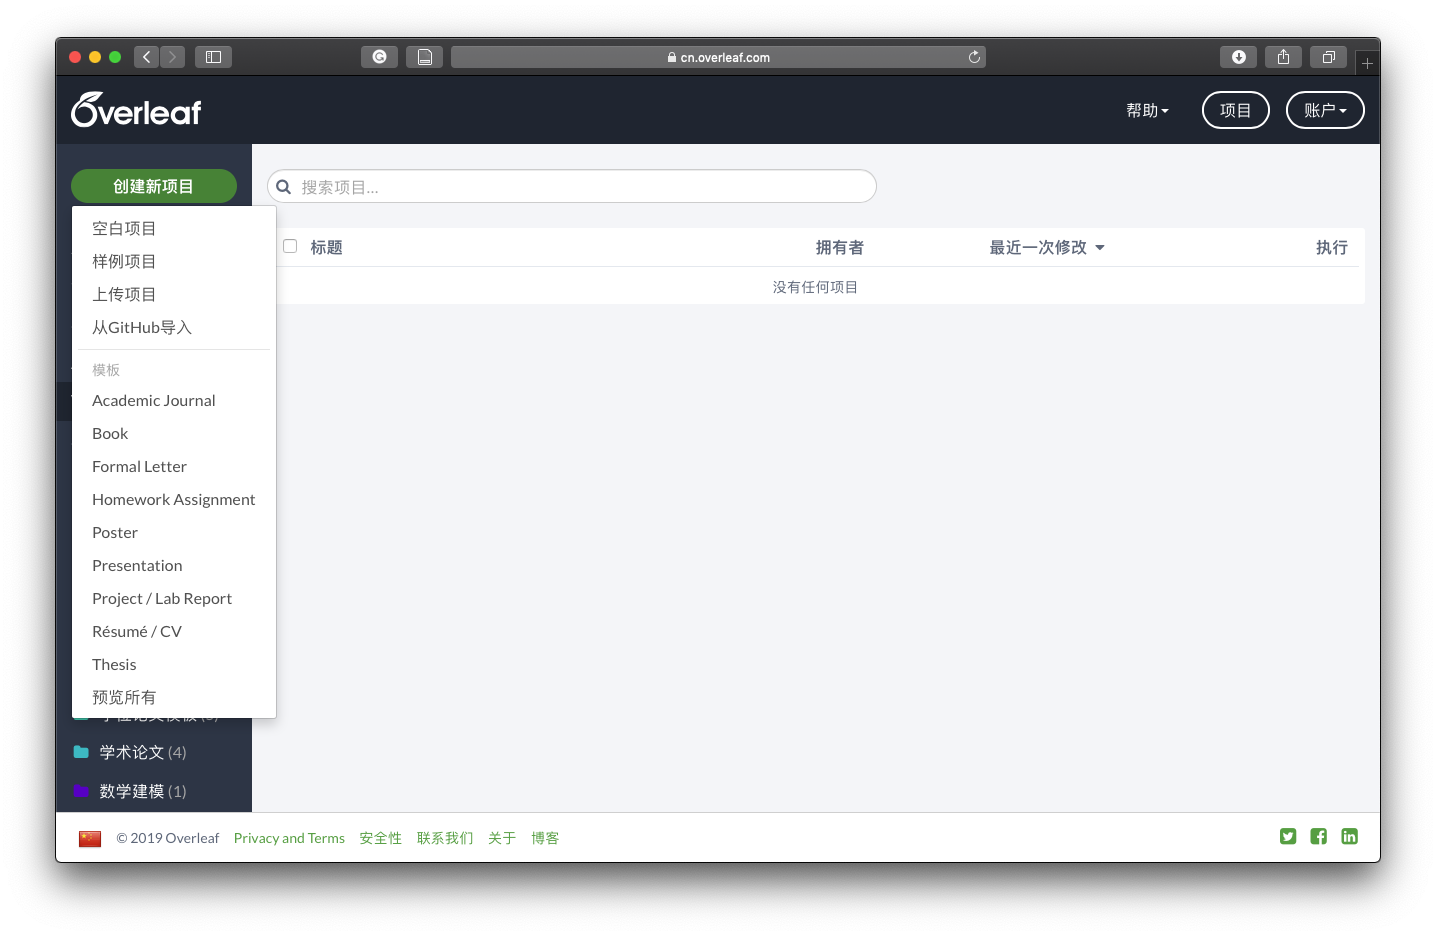
\includegraphics{/figure/newproject}
\caption{新建项目}
\end{figure}

登陆后,在左上角可以看到创建新项目

出了空白项目和上传项目之外,Overleaf有丰富的模板资源:
\url{https://cn.overleaf.com/latex/templates}

另外,还支持从GitHub导入模板.

\hypertarget{section-4}{%
\section{个人写作}\label{section-4}}

项目建好后,界面和其他的tex客户端几乎没有区别.
左侧是tex的源文件,右侧是生成的pdf文件.

\hypertarget{section-5}{%
\section{邀请合作者}\label{section-5}}

右上角可以看到一个 共享 的功能,点击可以通过链接分享项或者通过账号邀请(免费用户只有1个合作者限制).

接下来就可以一起编写文章.

\hypertarget{section-6}{%
\section{论文投递}\label{section-6}}

论文写完后,右上角有 submit 功能,可以直接提交到期刊(现在已接入的较少).

\hypertarget{section-7}{%
\chapter{特色功能展示}\label{section-7}}

\hypertarget{section-8}{%
\section{本地和服务器同步}\label{section-8}}

\hypertarget{section-9}{%
\section{合作编辑}\label{section-9}}

\hypertarget{section-10}{%
\section{历史版本}\label{section-10}}

\hypertarget{section-11}{%
\section{参考文献整合}\label{section-11}}

\hypertarget{section-12}{%
\chapter{缺陷和不足}\label{section-12}}

\hypertarget{section-13}{%
\section{订阅费用}\label{section-13}}

\url{https://www.overleaf.com/user/subscription/plans}

\hypertarget{section-14}{%
\section{常用符号少}\label{section-14}}

\hypertarget{section-15}{%
\chapter{示例项目}\label{section-15}}

这里通过链接分享一些示例项目.

beamer的示例项目:
\url{https://cn.overleaf.com/read/tpzfjkmsfwkw}

\hypertarget{section-16}{%
\chapter{其他工具}\label{section-16}}

这里介绍一些可以提高LaTeX写作效率的其他工具

\hypertarget{section-17}{%
\section{公式}\label{section-17}}

mathpix

可以很方便的将图片公式转成LaTex形式,手写笔记不太乱的话也是可以识别的.

\url{https://mathpix.com}

\hypertarget{section-18}{%
\section{表格}\label{section-18}}

在LaTeX中插入表格并不是很简单的一件事,尤其是当表头需要合并单元格时.
这里介绍一些可以提高输入表格效率的工具.

\hypertarget{xtable}{%
\subsection{xtable包}\label{xtable}}

在R中进行模拟时,将结果输出至LaTeX可以利用这个包中的xtable函数.

\url{https://cran.r-project.org/web/packages/xtable/index.html}

\begin{Shaded}
\begin{Highlighting}[]
\NormalTok{xtable}\OperatorTok{::}\KeywordTok{xtable}\NormalTok{(}\KeywordTok{matrix}\NormalTok{(}\KeywordTok{rnorm}\NormalTok{(}\DecValTok{12}\NormalTok{),}\DecValTok{3}\NormalTok{,}\DecValTok{4}\NormalTok{))}
\end{Highlighting}
\end{Shaded}

\begin{verbatim}
## % latex table generated in R 3.6.0 by xtable 1.8-4 package
## % Mon Jun  3 11:03:52 2019
## \begin{table}[ht]
## \centering
## \begin{tabular}{rrrrr}
##   \hline
##  & 1 & 2 & 3 & 4 \\ 
##   \hline
## 1 & -0.59 & 0.84 & -1.28 & 0.84 \\ 
##   2 & -0.99 & 0.30 & -0.93 & 0.01 \\ 
##   3 & 0.42 & -0.12 & 0.66 & 0.51 \\ 
##    \hline
## \end{tabular}
## \end{table}
\end{verbatim}

这样我们直接粘贴到LaTeX中就可以了.

但是,这还不够.每次都要复制粘贴仍然很麻烦,而且如果表格的行名、列名有特定的格式,并不能直接粘贴结果(macOS下可以支持选择矩形区域修改).

我们可以利用LaTeX的\textbackslash{}input\{\}指令,完成更酷的操作.

大致流程就是在R中将xtable的输出结果写入文本文件``tableXXXX.tex'',然后在tex中需要插入表格的地方\textbackslash{}input\{tableXXXX.tex\}.

这样我们每次要把R新计算出来的表格更新到tex中,只需要重新编译一次即可.

关于复杂表头的设计,可以参考这个回答:

\url{https://stackoverflow.com/questions/15036754/r-package-xtable-how-to-create-a-latextable-with-multiple-rows-and-columns-from}

比如这样:

\begin{Shaded}
\begin{Highlighting}[]
\CommentTok{#https://stackoverflow.com/questions/15036754/r-package-xtable-how-to-create-a-latextable-with-multiple-rows-and-columns-from}

\CommentTok{#setwd()}

\KeywordTok{library}\NormalTok{(xtable)}

\NormalTok{C =}\StringTok{ }\NormalTok{(}\KeywordTok{rep}\NormalTok{(}\DecValTok{0}\OperatorTok{:}\DecValTok{5}\NormalTok{,}\DecValTok{2}\NormalTok{))}
\NormalTok{n =}\StringTok{ }\KeywordTok{rep}\NormalTok{(}\KeywordTok{c}\NormalTok{(}\DecValTok{200}\NormalTok{,}\DecValTok{300}\NormalTok{),}\DataTypeTok{each=}\DecValTok{6}\NormalTok{)}

\NormalTok{data =}\StringTok{ }\KeywordTok{matrix}\NormalTok{(}\KeywordTok{runif}\NormalTok{(}\DecValTok{6}\OperatorTok{*}\DecValTok{12}\NormalTok{),}\DecValTok{12}\NormalTok{,}\DecValTok{6}\NormalTok{)}
\NormalTok{data =}\StringTok{ }\KeywordTok{round}\NormalTok{(data,}\DecValTok{3}\NormalTok{)}
\NormalTok{df =}\KeywordTok{data.frame}\NormalTok{(}\KeywordTok{c}\NormalTok{(}\KeywordTok{replicate}\NormalTok{(}\DecValTok{6}\NormalTok{,}\StringTok{"200"}\NormalTok{),}\KeywordTok{replicate}\NormalTok{(}\DecValTok{6}\NormalTok{,}\StringTok{"300"}\NormalTok{)),C,}\KeywordTok{cbind}\NormalTok{(data[,}\DecValTok{1}\OperatorTok{:}\DecValTok{3}\NormalTok{],}\KeywordTok{rep}\NormalTok{(}\StringTok{""}\NormalTok{,}\DecValTok{12}\NormalTok{),data[,}\DecValTok{4}\OperatorTok{:}\DecValTok{6}\NormalTok{]))}
\CommentTok{# only needed if first column consists of numbers}
\NormalTok{df[[}\DecValTok{1}\NormalTok{]] <-}\StringTok{ }\KeywordTok{as.character}\NormalTok{(df[[}\DecValTok{1}\NormalTok{]])}
\NormalTok{rle.lengths <-}\StringTok{ }\KeywordTok{rle}\NormalTok{(df[[}\DecValTok{1}\NormalTok{]])}\OperatorTok{$}\NormalTok{lengths}
\NormalTok{first <-}\StringTok{ }\OperatorTok{!}\KeywordTok{duplicated}\NormalTok{(df[[}\DecValTok{1}\NormalTok{]])}
\NormalTok{df[[}\DecValTok{1}\NormalTok{]][}\OperatorTok{!}\NormalTok{first] <-}\StringTok{ ""}

\CommentTok{# define appearance of \textbackslash{}multirow}
\NormalTok{df[[}\DecValTok{1}\NormalTok{]][first] <-}
\StringTok{  }\KeywordTok{paste0}\NormalTok{(}\StringTok{"}\CharTok{\textbackslash{}\textbackslash{}}\StringTok{multirow\{"}\NormalTok{, rle.lengths, }\StringTok{"\}\{*\}\{\{"}\NormalTok{, df[[}\DecValTok{1}\NormalTok{]][first], }\StringTok{"\}\}"}\NormalTok{)}
\NormalTok{addtorow <-}\StringTok{ }\KeywordTok{list}\NormalTok{()}
\NormalTok{addtorow}\OperatorTok{$}\NormalTok{pos <-}\StringTok{ }\KeywordTok{list}\NormalTok{(}\DecValTok{0}\NormalTok{, }\DecValTok{0}\NormalTok{, }\DecValTok{0}\NormalTok{)}
\NormalTok{addtorow}\OperatorTok{$}\NormalTok{command <-}\StringTok{ }\KeywordTok{c}\NormalTok{(}\StringTok{"}\CharTok{\textbackslash{}\textbackslash{}}\StringTok{multirow\{2\}*\{$n$\} &}\CharTok{\textbackslash{}\textbackslash{}}\StringTok{multirow\{2\}*\{$C$\}& }\CharTok{\textbackslash{}\textbackslash{}}\StringTok{multicolumn\{3\}\{c\}\{The homoscedastic cases\}&& }\CharTok{\textbackslash{}\textbackslash{}}\StringTok{multicolumn\{3\}\{c\}\{The heteroscedastic cases\} }\CharTok{\textbackslash{}\textbackslash{}\textbackslash{}\textbackslash{}\textbackslash{}n}\StringTok{"}\NormalTok{,}
                      \StringTok{" }\CharTok{\textbackslash{}\textbackslash{}}\StringTok{cline\{3-5\}     }\CharTok{\textbackslash{}\textbackslash{}}\StringTok{cline\{7-9\} "}\NormalTok{,}
                      \StringTok{"&& $}\CharTok{\textbackslash{}\textbackslash{}}\StringTok{tau=0.25$ & $}\CharTok{\textbackslash{}\textbackslash{}}\StringTok{tau=0.5$ & $}\CharTok{\textbackslash{}\textbackslash{}}\StringTok{tau=0.75$ && $}\CharTok{\textbackslash{}\textbackslash{}}\StringTok{tau=0.25$ & $}\CharTok{\textbackslash{}\textbackslash{}}\StringTok{tau=0.5$ & $}\CharTok{\textbackslash{}\textbackslash{}}\StringTok{tau=0.75$ }\CharTok{\textbackslash{}\textbackslash{}\textbackslash{}\textbackslash{}\textbackslash{}n}\StringTok{"}\NormalTok{)}
\KeywordTok{xtable}\NormalTok{(df,}\DataTypeTok{digits =} \KeywordTok{c}\NormalTok{(}\DecValTok{0}\NormalTok{,}\DecValTok{0}\NormalTok{,}\DecValTok{0}\NormalTok{,}\KeywordTok{rep}\NormalTok{(}\DecValTok{2}\NormalTok{,}\DecValTok{3}\NormalTok{),}\DecValTok{0}\NormalTok{,}\KeywordTok{rep}\NormalTok{(}\DecValTok{2}\NormalTok{,}\DecValTok{3}\NormalTok{))}
\NormalTok{       ,}\DataTypeTok{caption =} \StringTok{"测试"}
\NormalTok{       ,}\DataTypeTok{align =} \StringTok{"cccccccccc"}  \CommentTok{# align and put a vertical line (first "l" again represents column of row numbers)}
\NormalTok{       ,}\DataTypeTok{label =} \StringTok{"tab::test"}
\NormalTok{       ,}\DataTypeTok{hline.after=}\OtherTok{NULL}\NormalTok{, }\CommentTok{#We don't need hline; we use booktabs}
       \DataTypeTok{floating=}\OtherTok{TRUE} \CommentTok{# whether \textbackslash{}begin\{Table\} should be created (TRUE) or not (FALSE)}
\NormalTok{) ->}\StringTok{ }\NormalTok{outtable}

\CommentTok{#cat(}
  \KeywordTok{print}\NormalTok{(outtable,}
          \DataTypeTok{hline.after =} \KeywordTok{c}\NormalTok{(}\OperatorTok{-}\DecValTok{1}\NormalTok{,}\DecValTok{0}\NormalTok{,}\KeywordTok{nrow}\NormalTok{(outtable),}\KeywordTok{nrow}\NormalTok{(outtable)}\OperatorTok{-}\DecValTok{6}\NormalTok{),}
          \CommentTok{#booktabs = TRUE,}
          \DataTypeTok{sanitize.text.function =}\NormalTok{ force }\CommentTok{# Important to treat content of first column as latex function}
\NormalTok{          ,}\DataTypeTok{caption.placement =} \StringTok{"top"} \CommentTok{#"top", NULL}
\NormalTok{          ,}\DataTypeTok{add.to.row =}\NormalTok{ addtorow,}\DataTypeTok{include.colnames =} \OtherTok{FALSE}\NormalTok{,}\DataTypeTok{include.rownames =} \OtherTok{FALSE}\NormalTok{)}
\end{Highlighting}
\end{Shaded}

\begin{verbatim}
## % latex table generated in R 3.6.0 by xtable 1.8-4 package
## % Mon Jun  3 11:03:52 2019
## \begin{table}[ht]
## \centering
## \caption{测试} 
## \label{tab::test}
## \begin{tabular}{ccccccccc}
##   \hline
##   \multirow{2}*{$n$} &\multirow{2}*{$C$}& \multicolumn{3}{c}{The homoscedastic cases}&& \multicolumn{3}{c}{The heteroscedastic cases} \\
##      \cline{3-5}     \cline{7-9}  && $\tau=0.25$ & $\tau=0.5$ & $\tau=0.75$ && $\tau=0.25$ & $\tau=0.5$ & $\tau=0.75$ \\
##  \hline
## \multirow{6}{*}{{200}} & 0 & 0.273 & 0.021 & 0.453 &  & 0.549 & 0.768 & 0.305 \\ 
##    & 1 & 0.592 & 0.297 & 0.478 &  & 0.036 & 0.513 & 0.202 \\ 
##    & 2 & 0.806 & 0.802 & 0.932 &  & 0.228 & 0.022 & 0.176 \\ 
##    & 3 & 0.851 & 0.557 & 0.97 &  & 0.121 & 0.842 & 0.391 \\ 
##    & 4 & 0.8 & 0.501 & 0.272 &  & 0.217 & 0.851 & 0.609 \\ 
##    & 5 & 0.905 & 0.171 & 0.635 &  & 0.416 & 0.515 & 0.507 \\ 
##    \hline
## \multirow{6}{*}{{300}} & 0 & 0.41 & 0.945 & 0.522 &  & 0.697 & 0.442 & 0.296 \\ 
##    & 1 & 0.059 & 0.136 & 0.732 &  & 0.428 & 0.716 & 0.69 \\ 
##    & 2 & 0.356 & 0.88 & 0.972 &  & 0.863 & 0.596 & 0.007 \\ 
##    & 3 & 0.13 & 0.433 & 0.56 &  & 0.653 & 0.803 & 0.169 \\ 
##    & 4 & 0.175 & 0.344 & 0.713 &  & 0.516 & 0.395 & 0.289 \\ 
##    & 5 & 0.833 & 0.564 & 0.887 &  & 0.957 & 0.109 & 0.8 \\ 
##    \hline
## \end{tabular}
## \end{table}
\end{verbatim}

\begin{Shaded}
\begin{Highlighting}[]
    \CommentTok{#,file = "table.tex")}
\end{Highlighting}
\end{Shaded}

也支持生成html的形式.

\hypertarget{excel2latex}{%
\subsection{Excel2LaTeX}\label{excel2latex}}

可以在Excel中合并好单元格,导出tex的表格.

\url{https://github.com/krlmlr/Excel2LaTeX/releases}

\hypertarget{latex}{%
\subsection{LaTeX中合并单元格}\label{latex}}

\url{http://www.tablesgenerator.com/\#}

\hypertarget{section-19}{%
\chapter{一些模板}\label{section-19}}

\hypertarget{section-20}{%
\section{学位论文模板}\label{section-20}}

\url{https://github.com/ustctug/awesome-latex-thesis}

\hypertarget{elegantlatex}{%
\section{ElegantLaTeX}\label{elegantlatex}}

\url{https://github.com/ElegantLaTeX}

\hypertarget{beamer}{%
\section{beamer主题}\label{beamer}}

\url{http://deic.uab.es/~iblanes/beamer_gallery/index_by_theme.html}

\url{https://www.namsu.de/latex/themes/outer.html}

\cleardoublepage

\hypertarget{appendix-}{%
\appendix \addcontentsline{toc}{chapter}{\appendixname}}


\hypertarget{sound}{%
\chapter{余音绕梁}\label{sound}}

呐,到这里朕的书差不多写完了,但还有几句话要交待,所以开个附录,再啰嗦几句,各位客官稍安勿躁、扶稳坐好。

\bibliography{book.bib,packages.bib}

\backmatter
\printindex

\end{document}
